
% Template by Arnau, based on:
%%%%%%%%%%%%%%%%%%%%%%%%%%%%%%%%%%%%%%%%%
%
% Beamer Presentation
% LaTeX Template
% Version 1.0 (10/11/12)
% This template has been downloaded from:
% http://www.LaTeXTemplates.com
% License:
% CC BY-NC-SA 3.0 (http://creativecommons.org/licenses/by-nc-sa/3.0/)
%%%%%%%%%%%%%%%%%%%%%%%%%%%%%%%%%%%%%%%%%


%----------------------------------------------------------------------------------------
%	PACKAGES AND THEMES
%----------------------------------------------------------------------------------------

\documentclass[5pt]{beamer}
\usefonttheme{serif}
%% serif
%% professionalfonts
%% structurebold
%% structureitalicserif
%% structuresmallcapsserif

\mode<presentation> {

\usetheme{Boadilla}

% As well as themes, the Beamer class has a number of color themes
% for any slide theme. Uncomment each of these in turn to see how it
% changes the colors of your current slide theme.

% \usecolortheme{albatross}
%\usecolortheme{beaver}
%\usecolortheme{beetle}
%\usecolortheme{crane}
% \usecolortheme{dolphin}
%\usecolortheme{dove}
%\usecolortheme{fly}
%\usecolortheme{lily}
%\usecolortheme{orchid}
%\usecolortheme{rose}
%\usecolortheme{seagull}
\usecolortheme{seahorse}  % The them I usually use, because it resembles the PSI template.
% \usecolortheme{whale}
%\usecolortheme{wolverine}

%\setbeamertemplate{footline} % To remove the footer line in all slides uncomment this line
% \setbeamertemplate{footline}[page number] % To replace the footer line in all slides with a simple slide count uncomment this line
}

\setbeamertemplate{sections/subsections in toc}[sections numbered]  % Controls style of number in the table of contents.

% Packages:
\usepackage{pgfgantt}
\usepackage{colortbl}
\usepackage{pifont}
\usepackage{adjustbox}
\usepackage{algorithm}
\usepackage{algpseudocode}
\usepackage{amsmath,amsfonts,amsthm,amssymb}
\usepackage{animate}
\usepackage{appendixnumberbeamer}
\usepackage{booktabs} % Allows the use of \toprule, \midrule and \bottomrule in tables
\usepackage{cancel}
%\usepackage{dutchcal}
% \usepackage{enumitem}
\usepackage[shortlabels]{enumitem}
\usepackage{float}
\usepackage{graphicx} % Allows including images
\usepackage{hhline}
\usepackage{listings}
% Theme choice
% \usetheme{AnnArbor}
% Required package
\usepackage{caption}
 %so that the captions are numerated
\setbeamertemplate{caption}[numbered]
\lstset{
  language=Python,
  basicstyle=\ttfamily,
  mathescape
}
\lstdefinestyle{CppStyle}{
  language=C++,
  basicstyle=\ttfamily,
  keywordstyle=\color{blue},
  commentstyle=\color{green!60!black},
  stringstyle=\color{orange}
}
\usepackage{mathtools}
\usepackage{multicol}
\usepackage{multimedia}
\usepackage[authoryear]{natbib}
\usepackage{scrextend}
\usepackage{pdfpages}
\changefontsizes{8pt}
\usepackage{siunitx}
\usepackage{soul}
\usepackage{tikz}
\usetikzlibrary{mindmap, trees, arrows, shapes, backgrounds, matrix, decorations.pathreplacing, decorations.pathmorphing, positioning, arrows.meta,plotmarks, calc}
\usepackage{verbatim}
\usepackage{xmpmulti}

% \bibliographystyle{unsrt}  % This style cites with numbers, e.g. [2]
\bibliographystyle{unsrtnat}  % This style cites with names, e.g. [Adelmann, 2019]


%%%%%%%%%%%%%%%%%%%%%%%%%%%%%%%%%
% Tikz stuff:
\usetikzlibrary{positioning}
\usetikzlibrary{patterns}
\usetikzlibrary{shapes}
\usetikzlibrary{matrix, arrows,decorations.pathmorphing}
\usetikzlibrary{decorations.markings}
\usetikzlibrary{fadings}
\usetikzlibrary{arrows.meta,bending}
\usepackage{tikzscale}
%%%%%%%%%%%%%%%%%%%%%%%%%%%%%%%%%
%%%%%%%%%%%%%%%%%%%%%%%%%%%%%%%%%


\setbeamertemplate{navigation symbols}{}  % Remove navigation symbols
\setbeamersize{text margin left=1cm,text margin right=1cm}

%% Maths definitions.
\DeclareMathOperator*{\argmin}{arg\,min}
\DeclareMathOperator*{\supp}{supp}
\DeclareMathOperator*{\Var}{\mathrm{Var}}
\DeclareMathOperator*{\Cov}{\mathrm{Cov}}
\DeclareMathOperator*{\E}{\mathbb{E}}
\DeclareMathOperator*{\MSE}{\text{MSE}}
\DeclareMathOperator*{\sgn}{\text{sgn}}
\DeclareMathOperator*{\Epsilon}{\mathcal{E}}
\DeclareMathOperator*{\bigO}{\mathcal{O}}
\DeclareMathOperator*{\smalls}{s}
\newcommand{\mvec}[1]{\boldsymbol{#1}}
\newcommand\underrel[2]{\mathrel{\mathop{#2}\limits_{#1}}}

%----------------------------------------------------------------------------------------
%	TITLE PAGE
%----------------------------------------------------------------------------------------

%%%%%%%%%%%%%%%%%%%%%%%%%%%%%%%%%%%%%%%%%
% Enter here author information:
\title[Electromagnetic Simulation]{Performance portable FDTD Implementation} % The short title appears at the bottom of every slide, the full title is only on the title page.

\author{\textbf{Manuel Winkler}, S. Mayani, A. Adelmann}
\institute[PSI]{
AMAS Group, LSM\\ % Your institution for the title page.
}
\date{\today}

\def \myEmail {flaschenholz@protonmail.ch}
%%%%%%%%%%%%%%%%%%%%%%%%%%%%%%%%%%%%%%%

\newcommand{\frametitlepsi}[1]{\frametitle{\hspace{0.8cm}
\includegraphics[width=1.5cm]{logos/PSI.pdf}\hspace{1.1cm} #1}}

\begin{document}
\setbeamertemplate{caption}{\raggedright\insertcaption\par}
\def\vfilll{\vskip 0pt plus 1filll minus 0pt }
\begin{frame}
  % Title page image:
  \vspace{0.3cm}
  \begin{adjustbox}{width=\paperwidth, center}
    \begin{tikzpicture}
      \centering
      \filldraw[fill=lightgray!40!white, draw = none] (0,0) rectangle (3.3,0.5\textheight);
      % Logos:
      \node[anchor=south west,inner sep=0] at (0.4,3.4)
           {
\includegraphics[width=2.5cm]{logos/PSI.pdf}};
      \node[anchor=south west,inner sep=0] at (0.5,1.8)
           {
\includegraphics[width=2.4cm]{logos/eth_logo_kurz_pos.eps}};
    \end{tikzpicture}
    \begin{tikzpicture}
      \node (heli) [anchor=south west,inner sep=0] at (0,0)
            {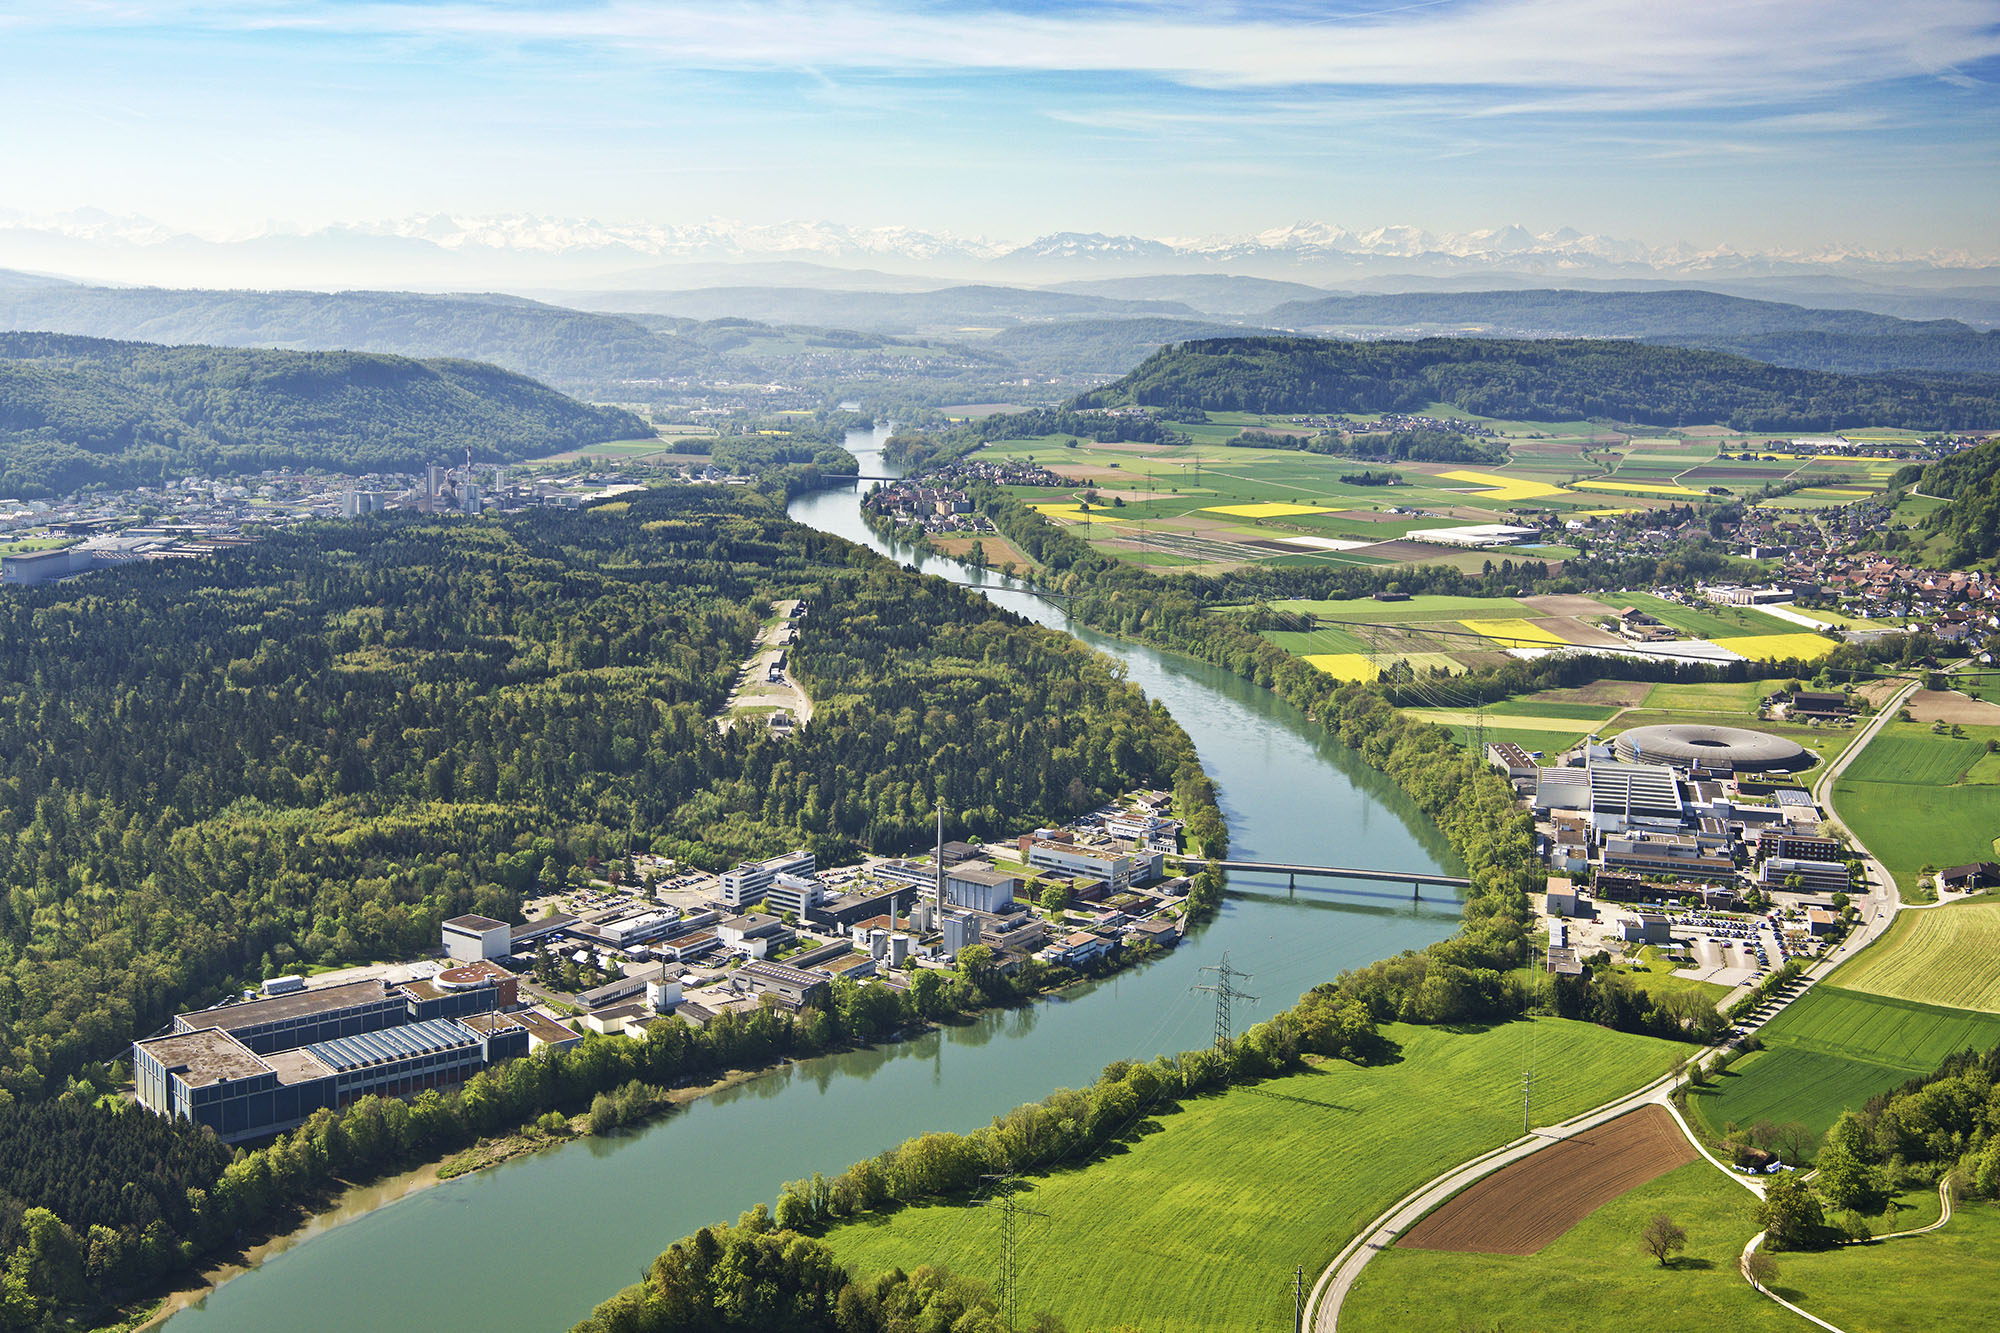
\includegraphics[height=0.5\textheight]{logos/PSI_helicopter}};
      \node [anchor=south west, inner sep = 1,fill=white, opacity=0.8] at (3.5, 0.0)
            {\tiny WIR SCHAFFEN WISSEN - HEUTE FÜR MORGEN};
    \end{tikzpicture}
    
\begin{tikzpicture}
      \filldraw[fill=lightgray!40!white, draw = none] (0,0) rectangle (1,0.5\textheight);
    \end{tikzpicture}
  \end{adjustbox}
  \vspace{0.1cm}\\
  {\usebeamerfont{subtitle} \footnotesize \insertauthor\, ::  \insertinstitute}
  \vspace{0.4cm}
  {\usebeamerfont{title} \LARGE \inserttitle}\\
  \vspace{0.4cm}
  {\usebeamerfont{subtitle} \footnotesize \insertdate}\\
  \vfilll
  \null\hfill\tiny Contact: \url{\myEmail}
\end{frame}

% Table of contents slide, comment this block out to remove it.
\begin{frame}[noframenumbering]
\frametitle{Overview}
\tableofcontents % Throughout your presentation, if you choose to use \section{} and \subsection{} commands, these will automatically be printed on this slide as an overview of your presentation.
\end{frame}

%----------------------------------------------------------------------------------------
%	PRESENTATION SLIDES
%----------------------------------------------------------------------------------------
\section{Governing equations}
\frame[noframenumbering]{\tableofcontents[currentsection]}
\begin{frame}
{\huge Field Update}
Define the four potential $A^\alpha = \left(\phi, \mathbf{A}\right)$ which evolves according to a wave equation:
\begin{align*}
\frac{\partial^2 A^\alpha}{\partial t^2} &= \Delta A^\alpha + S^\alpha \\
\text{where } S^\alpha &= \left(\rho, \mathbf{J}\right)
\end{align*}
\pause
The magnetic and electric fields can be evaluated with
\begin{align*}
\mathbf{E} &= -\nabla \phi - \frac{\partial \mathbf{A}}{\partial t} \\
\mathbf{B} &= \nabla \times \mathbf{A}
\end{align*}
\end{frame}
\section{Field Discretization}
\frame[noframenumbering]{\tableofcontents[currentsection]}
\begin{frame}
    \frametitle{Stencil}
Use a three-point second derivative stencil:
\begin{align*}
\frac{\partial^2 A^\alpha}{\partial \beta^2}(\vec{x}) \approx \frac{1}{\beta^2}\left(A^\alpha(\vec{x} + \beta)
 - 2 A^\alpha(\vec{x}) + A^\alpha(\vec{x} - \beta)\right)
\end{align*}
where $\beta$ is an arbitrary vector. \\
In a cartesian grid this simplifies to
\begin{align*}
    \frac{\partial^2 A^\alpha}{\partial x^2}(\vec{x}) \approx\frac{1}{\Delta x^2}\left(A^\alpha_{i+1,...} - 2 A^\alpha_{i,...} + A^\alpha_{i-1,...}\right)
\end{align*}
where $i$ is the index corresponding to the direction of $x_$

\end{frame}
\begin{frame}
\frametitle{FDTD Formulation}
  \begin{align*}
      \frac{\partial^2 \psi(x, y, z, t)}{\partial x^2} &=
      \frac{\psi^n_{i+1,j,k} - 2\psi^n_{i,j,k} + \psi^n_{i-1,j,k}}{\Delta x^2} \\
      \frac{\partial^2 \psi(x, y, z, t)}{\partial y^2} &=
      \frac{\psi^n_{i,j+1,k} - 2\psi^n_{i,j,k} + \psi^n_{i,j-1,k}}{\Delta y^2} \\
      \frac{\partial^2 \psi(x, y, z, t)}{\partial z^2} &=
      \frac{\psi^n_{i,j,k+1} - 2\psi^n_{i,j,k} + \psi^n_{i,j,k-1}}{\Delta z^2} \\
      \frac{\partial^2 \psi(x, y, z, t)}{\partial t^2} &=
      \frac{\psi^{n+1}_{i,j,k} - 2\psi^n_{i,j,k} + \psi^{n-1}_{i,j,k}}{\Delta t^2}
  \end{align*}
where $\psi$ represents a component of the four-potential.\\
\pause
\vspace{1cm}
Only unknown: $\psi^{n+1}_{i,j,k}$.
\end{frame}

\begin{frame}
    \frametitle{Accuracy Analysis}
Consider the one-dimensional analytical function around $x_0 = 0$
\begin{align*}
f(x) &= f(0) + x f'(0) + \frac{x^2}{2}f''(0) + \frac{x^3}{6}f'''(0) + \frac{x^4}{24}f''''(0) + \mathcal{O}(\Delta x^5)
\end{align*}
%\begin{align*}
%\frac{\partial^2 f}{\partial x^2} &= \frac{1}{\Delta x ^ 2}\left(f_{i + 1} - 2 f_{i} + f_{i - 1}\right)
%\end{align*}
\pause
We can add the evaluations at $\pm \Delta x$ and subtract twice the evaluation at $0$:
\begin{align*}
& f(\Delta x) + f(-\Delta x) - 2 f(0) = \\
\end{align*}
\pause
\begin{align*}
&  \hphantom{2} f(0) + \Delta x f'(0) + \frac{\Delta x ^ 2}{2}f''(0) + \frac{\Delta x ^ 3}{6}f'''(0) + \frac{\Delta x ^ 4}{24}f''''(0) + \mathcal{O}(\Delta x^5) \\
+& \hphantom{2} f(0) - \Delta x f'(0) + \frac{\Delta x ^ 2}{2}f''(0) - \frac{\Delta x ^ 3}{6}f'''(0) + \frac{\Delta x ^ 4}{24}f''''(0) + \mathcal{O}(\Delta x^5) \\
-& 2f(0) = \Delta x ^ 2 f''(0) +  \frac{\Delta x ^ 4}{12}f''''(0) + \mathcal{O}_E(\Delta x^6)
\end{align*}
where $\mathcal{O}_E$ implies only even terms.
\end{frame}
\begin{frame}
  {\huge Accuracy Analysis}
We therefore can see that 
\begin{align*}
\frac{1}{\Delta x^2} \left(f(\Delta x) + f(-\Delta x) - 2 f(0) \right) = f''(0) + \frac{\Delta x ^ 2}{12}f''''(0) + \mathcal{O}_E(\Delta x^4)
\end{align*}
approximates the second derivative of $f$ in $0$ with an error that is proportional to $f''''(0)$
\end{frame}
\begin{frame}
  {\huge First test case}
  Consider the 1D wave equation 
\begin{align*}
  \frac{\partial^2 f}{\partial x^2} &= \frac{\partial^2 f}{\partial t^2} \\ 
  f(t = 0, x) &= \sin(\pi x)
\end{align*}
with periodic boundary conditions defined on $[-1, 1]$.\\
\pause
Analytical solution:
\begin{align*}
f(t, x) &= \hphantom{\pi^4} \sin(\pi x)\cos(\pi t) \\
\text{implying } \frac{\partial^4 f}{\partial x^4}(0) &= \pi^4 \sin(\pi x) \cos(\pi t) \\
\text {and } f(1, x) &= -\sin(\pi x)
\end{align*}
Evolving this equation numerically with $\Delta x \neq \Delta t$ up to $t = 1$ yields
\begin{align*}
f_n(1, x) = -\sin(\pi x) + k\frac{\Delta t}{\Delta t}(\Delta x^2) + \mathcal{O}(\Delta x^4)
\end{align*}
\end{frame}
\begin{frame}
  {\huge First test case}
  Due to linearity, we can separate the evolution of the exact solution and the error.
  \begin{align*}
  f_n(1, x) &= -\sin(\pi x) + k\Delta x^2 + \mathcal{O}_E(\Delta x^4) \\
  \implies f_n(2, x) &= \hphantom{-} \sin(\pi x) - k\Delta x^2 + k\Delta x^2 + \mathcal{O}_{12}(\Delta x^4) + \mathcal{O}_E(\Delta x^4) \\
                     &= \hphantom{-} \sin(\pi x) + \mathcal{O}_{\hphantom{1}}(\Delta x^4) 
  \end{align*}
  \pause
  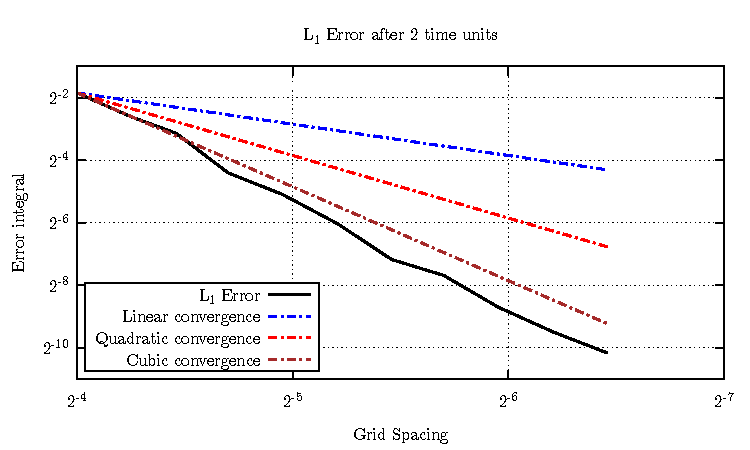
\includegraphics[width=\textwidth]{wave_error_cubic.pdf}
\end{frame}
\begin{frame}
  Additionally, in the case of $\Delta t = \Delta x$, the numerical wave operator
  \begin{align*}
  \frac{1}{\Delta x^2}\left(A^\alpha_{i+1,...} - 2 A^\alpha_{i,...} + A^\alpha_{i-1,...}\right) - \frac{1}{\Delta t^2}\left(A^\alpha_{...,n+1} - 2 A^\alpha_{...,n} + A^\alpha_{...,n-1}\right)
  \end{align*}
  reduces to zero for the exact solution
  \begin{align*}
    f(t, x) &= \sin(\pi x)\cos(\pi t)
  \end{align*}
  \pause
  because the even derivatives cancel:
  \begin{align*}
    \frac{\partial ^ {2n}f(t, x)}{\partial t^{2n}} &= \frac{\partial ^ {2n}f(t, x)}{\partial x^{2n}} = \pi ^ {2n}\sin(\pi x)\cos(\pi t)
  \end{align*}
\end{frame}
\begin{frame}
  {\huge Exact stepper}
  This results in machine precision accuracy for any grid spacing:
  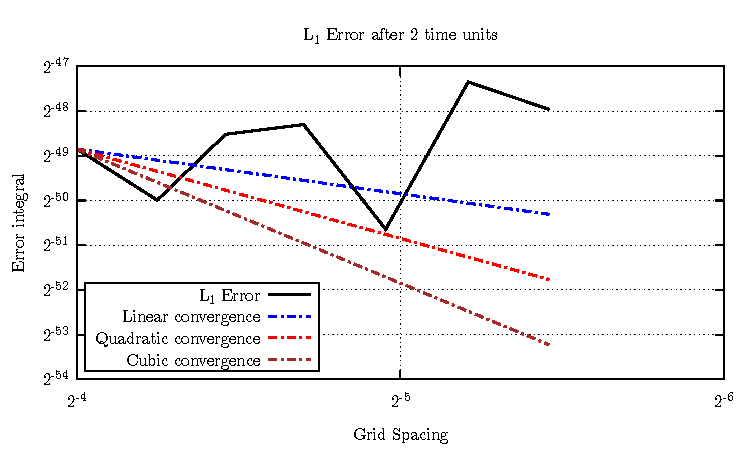
\includegraphics[width=\textwidth]{wave_error_machine.pdf}
\end{frame}
\begin{frame}
\frametitle{Boundary conditions}
Absorbing boundary conditions: Custom timestep rule on the boundary.

\vspace{1em}
Mathematical formulation:
\begin{align}
\left(\frac{\partial}{\partial x} - \frac{\partial}{\partial t}\right)\psi\bigg\rvert_{x = 0} &= 0 \text{ according to \cite{Mur1981}} \\
\vspace{2cm}\left(\frac{\partial^2}{\partial x \partial t} - \frac{\partial^2}{\partial t^2}\right)\psi\bigg\rvert_{x = 0} &= 0 \text{ according to according to \cite{fallahi2020mithra}} \label{fallahiabc}
\end{align}
\pause
Equation \ref{fallahiabc} can be used for boundaries with $\frac{\partial \psi}{\partial x}$, i.e. external fields:
\begin{align*}
\mathbf{E} &= \mathbf{e}_x \\
\matbf{\phi} &= x
\end{align*}
is a stationary solution only for \ref{fallahiabc}.
\end{frame}
\begin{frame}
\frametitle{Initial conditions}
For an initial source term
\begin{align*}
S &= \begin{bmatrix} \rho_0 \\ 0 \\ 0 \\ 0 \end{bmatrix}
\end{align*}
we solve the poisson equation
\begin{align*}
-\Delta \phi &= \rho_0
\end{align*}
\pause
For inital conditions with one moving particle:
\begin{align*}
\phi(\vec{r}, 0) &= \frac{q}{4 \pi(1 - \vec{\beta} \cdot \vec{n}) ||\vec{r} - \vec{R}(t_{ret})||} \\
\text{and } \mathbf{A}(\vec{r}, 0) &= \phi(r, 0) \vec{\beta}_{ret} \\ \\
\text{where } t_{ret} &= -||\vec{r} - \vec{R}(t_{ret})|| 
\end{align*}
\pause
For $p$ particles and $n$ gridpoints: $\mathcal{O}(p\cdot n)$!
\end{frame}
\section{Particle Discretization and Interpolation}
\frame[noframenumbering]{\tableofcontents[currentsection]}
\begin{frame}
  {\huge Particle Update}
  Lorentz Force:
\begin{align*}
  \vec{F_L} = q \mathbf{E} + q \vec{v} \times \mathbf{B} \\
\end{align*}
Lorentz acceleration:
\begin{align*}
  \vec{a_L} = \frac{q}{m_r} \mathbf{E} + q \vec{v} \times \mathbf{B} \\
  \text{where } m_r = \gamma m_0
\end{align*}
\end{frame}

\begin{frame}
  \frametitle{Particle timestep}
Boris update scheme with boosted $E$ and $B$: \cite{fallahi2020mithra}\\
\begin{align*}
  \left(r^m, \gamma \beta ^ {m - \frac{1}{2}}\right) &\rightarrow \left(r^{m + 1}, \gamma \beta ^ {m + \frac{1}{2}}\right) \\ \\
  \mathbf{t}_1 &= \gamma \mathbf{\beta}^{m - \frac 1 2} + \frac{e \Delta t_b \mathbf{E}_t^m}{2 m} \\
  &\vdots \\
  %\mathbf{t}_2 &= t_1 + \alpha t_1 \times \mathbf{B}_t^m \\
  %\mathbf{t}_3 &= t_1 + t_2 \times \frac{2 \alpha \mathbf{B}_t^m }{1 + \alpha^2 \mathbf{B}_t^m \cdot \mathbf{B}_t^m} \\
  %\gamma \mathbf{\beta}^{m + \frac 1 2} &= t_3 + \frac{e \Delta t_b \mathbf{E}_t^m}{2 m} \\
  \mathbf{r}^{m + 1} &= r^m + \frac{\Delta t_b \gamma \bm{\beta}^{m + \frac 1 2}}{\sqrt{1 + \lVert\gamma \mathbf{\beta}^{m + \frac 1 2}\rVert^2}} \\
  %\text{where } \alpha &= \frac{e \Delta t_b}{2m\sqrt{1 + \lVert t_1 \rVert^2}}
\end{align*}
\pause
Note that \\
\begin{align*}
\beta &= \frac{\gamma \beta}{\sqrt{1 + \lVert \gamma \beta \rVert^2}} \\
\gamma &= \sqrt{1 + \lVert \gamma \beta \rVert^2}
\end{align*}
\end{frame}
\begin{frame}
  \frametitle{Test of Boris Stepper}
  Setup: Shoot charged particle in constant $z$-aligned magnetic field\\
  \begin{minipage}{0.45\textwidth}
    \centering
  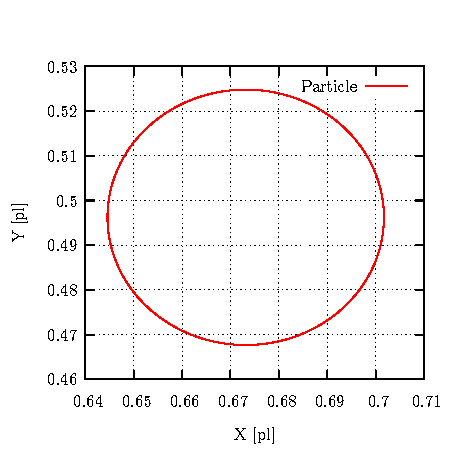
\includegraphics[width=\columnwidth]{trajectory_constant.pdf}
  \end{minipage}
  \hfill
  \begin{minipage}{0.45\textwidth}
  
  \begin{itemize}
    \item[$\cdot$] Traces a perfect circle
    \item[$\cdot$] Conserves energy up to machine precision
  \end{itemize}
\end{minipage}
\end{frame}
%\begin{frame}
%{\huge Particle to Grid interpolation}
%For an particle $p$ with position components
%\begin{align*}
%r &= \begin{bmatrix} \vdots \\ r_i \\ \vdots \end{bmatrix}, r_i = \lfloor \frac{r_i}{\Delta x_i}\rfloor \Delta x_i + \delta x_i = \alpha_i \Delta x_i + \delta x_i\\
%i \in \{0, N-1\} 
%\end{align*}
%the attribute $\rho$ is scattered to the $2^N$ nearest gridpoints with weights
%\begin{align*}
%\rho^p_{\alpha_0 + d_0,\alpha_1 + d_1,...} &= \prod_i^{N - 1} \left(d_i + \left[-\frac{\delta x_i}{\Delta x_i}\right]^{d_i}\right) \\
%\begin{bmatrix} \vdots \\ d_i \\ \vdots \end{bmatrix} &\in \{0, 1\}^N
%\end{align*}
%\end{frame}



\begin{frame}{Particle Discretization}
  Interpolation of a particle attribute to the grid: For a particle with position
  {\scriptsize
  \begin{align}
  p &= \begin{bmatrix} p_x \\ p_y \\ p_z \end{bmatrix} = \begin{bmatrix}
      \left \lfloor{\frac{p_x}{\Delta x}}\right \rfloor \Delta x + \delta_x \\
      \left \lfloor{\frac{p_y}{\Delta y}}\right \rfloor \Delta y + \delta_y \\ 
      \left \lfloor{\frac{p_z}{\Delta z}}\right \rfloor \Delta z + \delta_z \end{bmatrix} = 
  \begin{bmatrix} i \Delta x + \delta_x \\ j \Delta x + \delta_y \\ k \Delta x + \delta_z \end{bmatrix}
  \end{align}
  }%
  the Cloud-In-Cell interpolation is done as follows
  {\scriptsize
  \begin{align}
  \rho^p_{i+I,j+J,k+K} &= \rho\left(\frac{1}{2} + (-1)^I \bigg\rvert \frac{1}{2} - \frac{\delta x}{\Delta x} \bigg\rvert \right)
                              \left(\frac{1}{2} + (-1)^J \bigg\rvert \frac{1}{2} - \frac{\delta y}{\Delta y} \bigg\rvert \right)
                              \left(\frac{1}{2} + (-1)^K \bigg\rvert \frac{1}{2} - \frac{\delta z}{\Delta z} \bigg\rvert \right)
  \end{align}
  with $(I,J,K) \in \{0,1\}^3$.
  }%
  \end{frame}
  \begin{frame}
  \frametitle{Gathering field attributes}
  Interpolating field attributes to particles works analogously:
  {\scriptsize
  \begin{align*}
      \psi^p &= \sum_{I,I,K \in \{0,1\}^3} \psi \left(\frac{1}{2} + (-1)^I \bigg\rvert \frac{1}{2} - \frac{\delta x}{\Delta x} \bigg\rvert \right)
                                                \left(\frac{1}{2} + (-1)^J \bigg\rvert \frac{1}{2} - \frac{\delta y}{\Delta y} \bigg\rvert \right)
                                                \left(\frac{1}{2} + (-1)^K \bigg\rvert \frac{1}{2} - \frac{\delta z}{\Delta z} \bigg\rvert \right)
  \end{align*}
  }%
  \end{frame}
  \begin{frame}
  \frametitle{Current Deposition}
  Cloud-In-Cell deposition of current: 
  We define the deposition point $p^m$ as the midpoint between two adjacent timesteps:
  {\scriptsize
  \begin{align}
  p^m &= \begin{bmatrix} \frac{p_x^n + p_x^{n+1}}{2} \\ \frac{p_y^n + p_y^{n+1}}{2} \\ \frac{p_z^n + p_z^{n+1}}{2} \end{bmatrix} = 
  \begin{bmatrix} 
  \left \lfloor{\frac{p^m_x}{\Delta x}}\right \rfloor \Delta x + \delta_x \\ 
  \left \lfloor{\frac{p^m_y}{\Delta y}}\right \rfloor \Delta y + \delta_y \\ 
  \left \lfloor{\frac{p^m_z}{\Delta z}}\right \rfloor \Delta z + \delta_z \end{bmatrix}
  \end{align}
  }%
  {\scriptsize
  \begin{align}
  \mathbf{J}^p_{i+I,j+J,k+K} &= \rho\mathbf{v}\left(\frac{1}{2} + (-1)^I \bigg\rvert \frac{1}{2} - \frac{\delta x}{\Delta x} \bigg\rvert \right)
                                    \left(\frac{1}{2} + (-1)^J \bigg\rvert \frac{1}{2} - \frac{\delta y}{\Delta y} \bigg\rvert \right)
                                    \left(\frac{1}{2} + (-1)^K \bigg\rvert \frac{1}{2} - \frac{\delta z}{\Delta z} \bigg\rvert \right) \\
                                    \text{where } \mathbf{v} &= \frac{r^{m + 1} - r^{m - 1}}{2 \Delta t}
  \end{align}
  }%
  \pause
  If a particle travels across a cell boundary, this scheme violates
  {\scriptsize
  \begin{align}
  \nabla \cdot \mathbf{E} &= \rho
  \end{align}
  }%
  \end{frame}
  \begin{frame}
  \frametitle{Boris Correction}
  To satisfy
  \begin{align*}
  \nabla \cdot \mathbf{E} &= \rho
  \end{align*}
  we simply add a correction term equivalent to the negative error \cite{Lund2016}:
  \begin{align}
  \mathbf{E'} &= \mathbf{E} - \nabla\delta\phi \text{ with } \nabla \cdot \left(\nabla\delta\phi\right) = \nabla \cdot \mathbf{E} - \rho
  \end{align}
  \end{frame}
  \begin{frame}
  \frametitle{Zigzag Current Deposition}
  Alternatively change current deposition scheme: Particle motion from $p_1$ to $p_2$ is decomposed into two separate movements, $p_1$ to $p_r$ and $p_r$ to $p_2$ \cite{fallahi2020mithra}.
  {\scriptsize
  \begin{align*}
      x_r &= \min\left(\min(i_1\Delta x, i_2 \Delta x) + \Delta_x, \max\left(\min(i_1\Delta x, i_2 \Delta x), \frac{x_1 + x_2}{2}\right)\right)\\
      y_r &= \min\left(\min(j_1\Delta x, j_2 \Delta y) + \Delta_y, \max\left(\min(j_1\Delta y, j_2 \Delta y), \frac{y_1 + y_2}{2}\right)\right)\\
      z_r &= \min\left(\min(k_1\Delta x, k_2 \Delta z) + \Delta_z, \max\left(\min(k_1\Delta z, k_2 \Delta z), \frac{z_1 + z_2}{2}\right)\right)
  \end{align*}
  }%
  Then two Cloud-In-Cell interpolations of with points $\frac{p_1 + p_r}{2}$ and $\frac{p_r + p_2}{2}$ \cite{UMEDA200373} satisfy the conservation of current.
  \end{frame}

\begin{frame}
  
  \frametitle{Test of current deposition and field update}
  Idea: Compare simulated radiation to Larmor:
  \begin{align*}
    P &= \frac{q^2}{6\pi}\gamma^6(||\dot {\vec \beta}||^2 - ||\vec\beta \times \dot{\vec \beta}||^2)
  \end{align*}
  \begin{minipage}{0.45\textwidth}
    \centering
    \begin{figure}[h] 
      \centering
      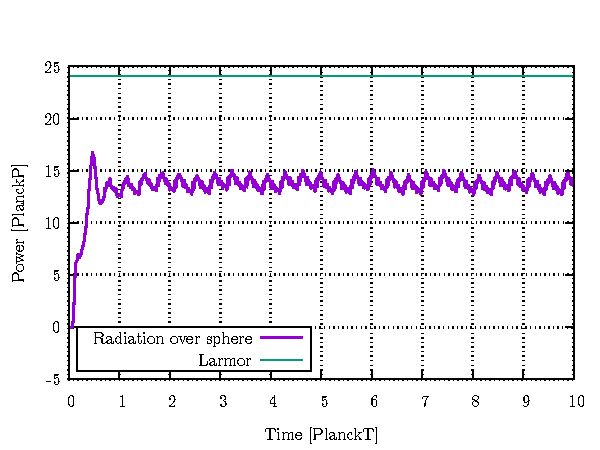
\includegraphics[width=\columnwidth]{radplot_badres.pdf}
      \caption{$\sigma_{init}$ = 0.02}
      \label{fig:bigvar}
    \end{figure}
  \end{minipage}
  \hfill
  \begin{minipage}{0.5\textwidth}
  
  Setup:
  \begin{itemize}
    \item[$\cdot$] Initialize particles with gaussian distribution
    \item[$\cdot$] Rotate particles around center with fixed speed.
  \end{itemize} 
  \pause
  Observations:
  \begin{itemize}
    \item[$\cdot$] Constant outward radiation
    \item[$\cdot$] Different particle trajectories interfere destructively
  \end{itemize}
\end{minipage}
\end{frame}
\begin{frame}
  \frametitle{Test of current deposition and field update}
  \begin{minipage}{0.45\textwidth}
    \begin{figure}[h]
      \centering
      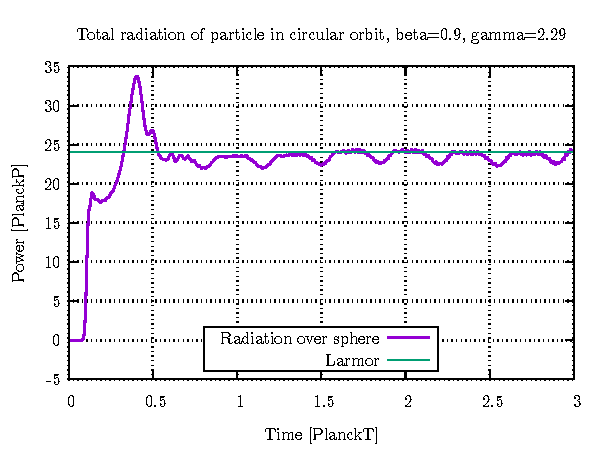
\includegraphics[width=\columnwidth]{radplot_goodres.pdf}
      \caption{$\sigma_{init}$ = 0.005}
      \label{fig:smallvar}
    \end{figure}
  \end{minipage}
  \hfill
  \begin{minipage}{0.5\textwidth}
  
  Setup:
  \begin{itemize}
    \item[\cdot] Initialize particles with gaussian distribution
    \item[\cdot] Rotate particles around center with fixed speed.
  \end{itemize} 
  Observations:
  \begin{itemize}
    \item[\cdot] Constant outward radiation
    \item[\cdot] Different particle trajectories interfere destructively
  \end{itemize}
\end{minipage}
\end{frame}
\begin{frame}
  \frametitle{Test of coupled field and particle update}
  \begin{minipage}{0.45\textwidth}
    \begin{figure}[h]
      \centering
      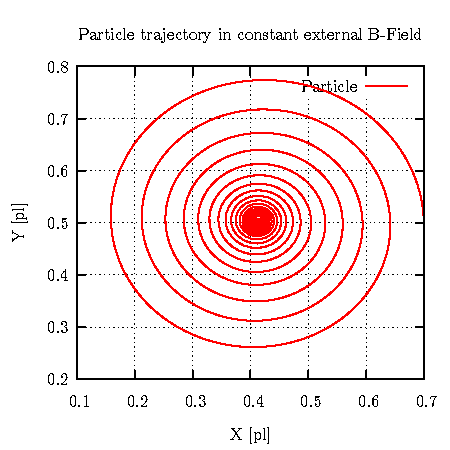
\includegraphics[width=\columnwidth]{trajectory_radiatinggood.pdf}
      \caption{$\sigma_{init}$ = 0.0}
      \label{fig:smallvar}
    \end{figure}
  \end{minipage}
  \hfill
  \begin{minipage}{0.5\textwidth}
  
  Setup:
  \begin{itemize}
    \item[\cdot] Initialize particles with gaussian distribution
    \item[\cdot] Let particles be guided by Lorentz force
  \end{itemize} 
  Observations:
  \begin{itemize}
    \item[\cdot] Particle progressively loses energy and spirals inward
  \end{itemize}
\end{minipage}


\end{frame}


\begin{frame}
  \frametitle{Test of coupled field and particle update}
  \begin{minipage}{0.45\textwidth}
    \begin{figure}[h]
      \centering
      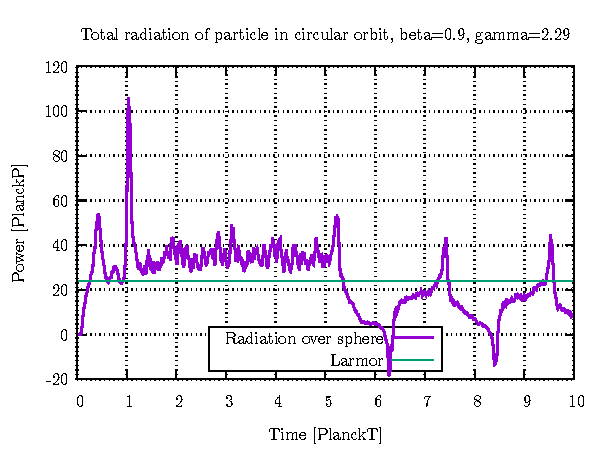
\includegraphics[width=\columnwidth]{radplot_lorentz.pdf}
      \caption{\sigma_{init} = 0.0}
      \label{fig:smallvar}
    \end{figure}
  \end{minipage}
  \hfill
  \begin{minipage}{0.5\textwidth}
  
  Setup:
  \begin{itemize}
    \item[\cdot] Initialize particles with gaussian distribution
    \item[\cdot] Let particles be guided by Lorentz force
  \end{itemize} 
  Observations:
  \begin{itemize}
    \item[\cdot] Constant outward radiation up until all energy is lost
  \end{itemize}
\end{minipage}
\end{frame}
\section{Outlook}
\frame[noframenumbering]{\tableofcontents[currentsection]}
\begin{frame}[fragile]
\frametitle{Undulators and Lorentz boosts}
Transformation of undulator fields:
\begin{align*}
\mathbf{B}_{lab}(\mathbf{r}) = \begin{bmatrix} 0 \\ B_0 \cosh{(k \cdot y_{lab})} \sin{(k \cdot z_{lab})} \\ B_0 \sinh{(k \cdot y_{lab})} \cos{(k \cdot z_{lab})} \end{bmatrix}
\end{align*}
\pause
\begin{align*}
  r_{lab} &= \mathbf{\Lambda}^{-1}(r_{bunch}) \\
  \mathbf{E}_{bunch} &= \gamma(\mathbf{E}_{lab} + \mathbf{v} \times \mathbf{B}_{lab}) - (\gamma - 1)\left(\mathbf{E}_{lab} \cdot \frac{\mathbf{v}}{||\mathbf{v}||}\right) \\
  \mathbf{B}_{bunch} &= \gamma(\mathbf{B}_{lab} - \mathbf{v} \times \mathbf{E}_{lab}) - (\gamma - 1)\left(\mathbf{B}_{lab} \cdot \frac{\mathbf{v}}{||\mathbf{v}||}\right) \\
  \text{or equivalently  } \mathbf{F}^{\alpha\beta}_{bunch} &= \mathbf{\Lambda}^\beta_\alpha \mathbf{F}^{\alpha \beta}_{lab}\mathbf{\Lambda}_\beta^\alpha
\end{align*}
%\end{frame}
%\begin{frame}[fragile]
In code:
\begin{lstlisting}[style=CppStyle]
{
  lorentzBoost<double> boost({0.0, 0.0, 0.99});
                                  //Lab to bunch frame
  ippl::Matrix<double, 4, 4> mat = boost.unprimedToPrimed();
}
\end{lstlisting}
\end{frame}
\begin{frame}
\frametitle{Resampling}
Assign weight $w_i$ to each particle $p_i$.
\pause
Resampling must conserve:
\begin{align*}
  \sum _{i = 1} ^ {N_{b}} w^b_i &= \sum _{j = 1} ^ {N_{a}} w^a_j
\end{align*}
The "true" quantity $q$ of particle $p_i$ is given by $\rho_i \cdot w_i$. \\
\pause
\vspace{1cm}
Preferrably also conserve 
\begin{align*}
\overline {\mathbf{r}} &= \sum _{i = 1} ^ {N}\frac{\mathbf{r_i}}{N} \text{    } \text{    (Center of mass)} \\
\sigma &= \sum _{i = 1} ^ {N}\frac{(\mathbf{r_i} - \overline {\mathbf{r}})}{N} \text{    } \text{    (Variance)} \\
\end{align*}
\end{frame}
\begin{frame}
\frametitle{Bibliography}
%\bibliographystyle{IEEEtran}
\bibliography{references}
\end{frame}
\end{document}
